\section{Рабочий проект}
\subsection{Классы, используемые при разработке сайта}

В результате разработки маркетплейса были реализованы классы и компоненты, обеспечивающие работоспособность системы. Спецификация классов и компонентов описана в этой главе. (таблица \ref{class:table}).

\subsubsection{Спецификация класса ClassController}

Этот класс предназначен для управления операциями, связанными с классами. Он включает методы для создания и получения всех классов.

\renewcommand{\arraystretch}{0.8}
\begin{xltabular}{\textwidth}{|X|p{2.5cm}|p{4.85cm}|p{4.85cm}|}
	\caption{Описание методов класса ClassController\label{classcontroller:table}}\\
	\hline Название метода & Область видимости & Тип значения & Описание \\
	\hline \endfirsthead
	\caption*{Продолжение таблицы \ref{classcontroller:table}}\\
	\hline Название метода & Область видимости & Тип значения & Описание \\
	\hline \endhead
	create & public & Promise & Создает новый класс на основе данных из тела запроса и возвращает его в формате JSON. \\
	\hline
	getAll & public & Promise & Возвращает список всех классов в формате JSON. \\
	\hline
\end{xltabular}
\renewcommand{\arraystretch}{1.0}

\subsubsection{Спецификация класса ItemController}

Этот класс управляет операциями, связанными с предметами. Он включает методы для создания, получения, поиска и удаления предметов, а также для работы с хранилищем.

\renewcommand{\arraystretch}{0.8}
\begin{xltabular}{\textwidth}{|X|p{2.5cm}|p{4.85cm}|p{4.85cm}|}
	\caption{Описание методов класса ItemController\label{itemcontroller:table}}\\
	\hline Название метода & Область видимости & Тип значения & Описание \\
	\hline \endfirsthead
	\caption*{Продолжение таблицы \ref{itemcontroller:table}}\\
	\hline Название метода & Область видимости & Тип значения & Описание \\
	\hline \endhead
	create & public & Promise & Создает новый предмет на основе данных из тела запроса и возвращает его в формате JSON. \\
	\hline
	getAll & public & Promise & Возвращает список всех предметов в формате JSON с учетом фильтров и пагинации. \\
	\hline
	getOne & public & Promise & Возвращает один предмет по его идентификатору. \\
	\hline
	search & public & Promise & Ищет предметы по их названию и возвращает результаты в формате JSON. \\
	\hline
	getStorage Items & public & Promise & Возвращает предметы из хранилища с учетом фильтров и пагинации. \\
	\hline
	getUserItems & public & Promise & Возвращает предметы пользователя из хранилища. \\
	\hline
	addItemTo Storage & public & Promise & Добавляет предмет в хранилище и возвращает его в формате JSON. \\
	\hline
	deleteItem & public & Promise & Удаляет предмет из хранилища по его идентификатору. \\
	\hline
	getAmmo InfosBy ItemId & public & Promise & Возвращает информацию о патронах для заданного предмета. \\
	\hline
\end{xltabular}
\renewcommand{\arraystretch}{1.0}

\subsubsection{Спецификация класса TypeController}

Этот класс управляет операциями, связанными с типами предметов. Он включает методы для создания и получения всех типов.

\renewcommand{\arraystretch}{0.8}
\begin{xltabular}{\textwidth}{|X|p{2.5cm}|p{4.85cm}|p{4.85cm}|}
	\caption{Описание методов класса TypeController\label{typecontroller:table}}\\
	\hline Название метода & Область видимости & Тип значения & Описание \\
	\hline \endfirsthead
	\caption*{Продолжение таблицы \ref{typecontroller:table}}\\
	\hline Название метода & Область видимости & Тип значения & Описание \\
	\hline \endhead
	create & public & Promise & Создает новый тип предмета на основе данных из тела запроса и возвращает его в формате JSON. \\
	\hline
	getAll & public & Promise & Возвращает список всех типов предметов в формате JSON. \\
	\hline
\end{xltabular}
\renewcommand{\arraystretch}{1.0}

\subsubsection{Спецификация класса UserController}

Этот класс управляет операциями, связанными с пользователями. Он включает методы для регистрации, аутентификации, изменения пароля и управления хранилищем.

\renewcommand{\arraystretch}{0.8}
\begin{xltabular}{\textwidth}{|X|p{2.5cm}|p{4.85cm}|p{4.85cm}|}
	\caption{Описание методов класса UserController\label{usercontroller:table}}\\
	\hline Название метода & Область видимости & Тип значения & Описание \\
	\hline \endfirsthead
	\caption*{Продолжение таблицы \ref{usercontroller:table}}\\
	\hline Название метода & Область видимости & Тип значения & Описание \\
	\hline \endhead
	registration & public & Promise & Регистрация нового пользователя с хешированным паролем и создание для него хранилища. \\
	\hline
	login & public & Promise & Аутентификация пользователя и генерация JWT токена. \\
	\hline
	check & public & Promise & Проверка JWT токена пользователя. \\
	\hline
	change Password & public & Promise & Изменение пароля пользователя. \\
	\hline
	createStorage & public & Promise & Создание нового хранилища для пользователя. \\
	\hline
	addItemTo Storage & public & Promise & Добавление предмета в хранилище пользователя. \\
	\hline
	getItems FromStorage & public & Promise & Получение предметов из хранилища с учетом фильтров и пагинации. \\
	\hline
	update Nicknames & public & Promise & Обновление никнеймов пользователя. \\
	\hline
\end{xltabular}
\renewcommand{\arraystretch}{1.0}

\subsubsection{Спецификация класса ItemStore}

Этот класс управляет состоянием предметов и их типов в приложении. Он включает методы для установки и получения типов, классов и предметов, а также для управления пагинацией.

\renewcommand{\arraystretch}{0.8}
\begin{xltabular}{\textwidth}{|X|p{2.5cm}|p{4.85cm}|p{4.85cm}|}
	\caption{Описание методов класса ItemStore\label{itemstore:table}}\\
	\hline Название метода & Область видимости & Тип значения & Описание \\
	\hline \endfirsthead
	\caption*{Продолжение таблицы \ref{itemstore:table}}\\
	\hline Название метода & Область видимости & Тип значения & Описание \\
	\hline \endhead
	setTypes & public & void & Устанавливает список типов предметов. \\
	\hline
	setClasses & public & void & Устанавливает список классов предметов. \\
	\hline
	setItems & public & void & Устанавливает список предметов. \\
	\hline
	setSelected Type & public & void & Устанавливает выбранный тип предмета и сбрасывает страницу на 1. \\
	\hline
	setSelected Class & public & void & Устанавливает выбранный класс предмета и сбрасывает страницу на 1. \\
	\hline
	setPage & public & void & Устанавливает текущую страницу. \\
	\hline
	setTotal Count & public & void & Устанавливает общее количество предметов. \\
	\hline
	get types & public & array & Возвращает список типов предметов. \\
	\hline
	get classes & public & array & Возвращает список классов предметов. \\
	\hline
	get items & public & array & Возвращает список предметов. \\
	\hline
	get selectedType & public & object & Возвращает выбранный тип предмета. \\
	\hline
	get selectedClass & public & object & Возвращает выбранный класс предмета. \\
	\hline
	get totalCount & public & number & Возвращает общее количество предметов. \\
	\hline
	get page & public & number & Возвращает текущую страницу. \\
	\hline
	get limit & public & number & Возвращает лимит предметов на странице. \\
	\hline
\end{xltabular}
\renewcommand{\arraystretch}{1.0}

\subsubsection{Спецификация класса UserStore}

Этот класс управляет состоянием аутентификации пользователя в приложении. Он включает методы для установки и получения состояния аутентификации и данных пользователя.

\renewcommand{\arraystretch}{0.8}
\begin{xltabular}{\textwidth}{|X|p{2.5cm}|p{4.85cm}|p{4.85cm}|}
	\caption{Описание методов класса UserStore\label{userstore:table}}\\
	\hline Название метода & Область видимости & Тип значения & Описание \\
	\hline \endfirsthead
	\caption*{Продолжение таблицы \ref{userstore:table}}\\
	\hline Название метода & Область видимости & Тип значения & Описание \\
	\hline \endhead
	setIsAuth & public & void & Устанавливает состояние аутентификации пользователя. \\
	\hline
	setUser & public & void & Устанавливает данные пользователя. \\
	\hline
	get isAuth & public & boolean & Возвращает состояние аутентификации пользователя. \\
	\hline
	get user & public & object & Возвращает данные пользователя. \\
	\hline
\end{xltabular}
\renewcommand{\arraystretch}{1.0}

\subsubsection{Спецификация компонента Profile}

Этот компонент предназначен для отображения и редактирования профиля пользователя, включая его игровые никнеймы и выставленные товары. Также он позволяет пользователю изменять пароль.

\renewcommand{\arraystretch}{0.8}
\begin{xltabular}{\textwidth}{|X|X|X|X|}
	\caption{Описание методов компонента Profile\label{profile:table}}\\
	\hline Название метода & Область видимости & Тип значения & Описание \\
	\hline \endfirsthead
	\caption*{Продолжение таблицы \ref{profile:table}}\\
	\hline Название метода & Область видимости & Тип значения & Описание \\
	\hline \endhead
	fetchData & private & async function & Асинхронный метод для получения данных пользователя и его предметов после инициализации компонента. \\
	\hline
	handleOpen ChangePassword Modal & private & void & Открывает модальное окно для изменения пароля. \\
	\hline
	handleClose ChangePassword Modal & private & void & Закрывает модальное окно для изменения пароля. \\
	\hline
	handleInput Change & private & function & Обрабатывает изменения в полях ввода никнеймов. \\
	\hline
	handleSave Nicknames & private & async function & Сохраняет изменения никнеймов пользователя. \\
	\hline
	handle DeleteItem & private & async function & Удаляет предмет из списка выставленных товаров пользователя. \\
	\hline
	useEffect & private & hook & Используется для выполнения побочных эффектов при инициализации компонента. \\
	\hline
\end{xltabular}
\renewcommand{\arraystretch}{1.0}

\subsubsection{Спецификация компонента Shop}

Этот компонент предназначен для отображения товаров, доступных для продажи, и включает функционал для фильтрации товаров по типам и классам. Также он позволяет пользователю выставлять товары на продажу.

\renewcommand{\arraystretch}{0.8}
\begin{xltabular}{\textwidth}{|X|X|X|X|}
	\caption{Описание методов компонента Shop\label{shopmethods:table}}\\
	\hline Название метода & Область видимости & Тип значения & Описание \\
	\hline \endfirsthead
	\caption*{Продолжение таблицы \ref{shopmethods:table}}\\
	\hline Название метода & Область видимости & Тип значения & Описание \\
	\hline \endhead
	handleSellItem & private & async function & Обрабатывает выставление товара на продажу, закрывая модальное окно после выполнения операции. \\
	\hline
	fetchData & private & async function & Асинхронный метод для получения типов товаров, классов товаров и товаров из хранилища после инициализации компонента. \\
	\hline
	useEffect & private & hook & Используется для выполнения побочных эффектов при инициализации компонента и последующих изменениях зависимостей (device.selected Type, device.selected Class, device.page, serverId). \\
	\hline
\end{xltabular}
\renewcommand{\arraystretch}{1.0}

\subsubsection{Спецификация компонента Auth}

Этот компонент отвечает за авторизацию и регистрацию пользователей в приложении. Он отображает соответствующие формы ввода и управляет процессом входа и регистрации пользователей.

\renewcommand{\arraystretch}{0.8}
\begin{xltabular}{\textwidth}{|X|X|X|X|}
	\caption{Описание методов компонента Auth\label{authmethods:table}}\\
	\hline Название метода & Область видимости & Тип значения & Описание \\
	\hline \endfirsthead
	\caption*{Продолжение таблицы \ref{authmethods:table}}\\
	\hline Название метода & Область видимости & Тип значения & Описание \\
	\hline \endhead
	click & private & async function & Обрабатывает нажатие кнопки "Войти" или "Зарегистрироваться", выполняет вход или регистрацию, устанавливает состояние пользователя как авторизованного и перенаправляет на главную страницу. \\
	\hline
\end{xltabular}
\renewcommand{\arraystretch}{1.0}


\subsection{Модульное тестирование}

Модульное тестирование – это процесс тестирования отдельных частей программы, называемых модулями, с целью убедиться, что они работают правильно. Каждый модуль обычно представляет собой небольшую часть общей программы, например, отдельную функцию или компонент. Модульное тестирование направлено на проверку правильности работы этих модулей в изоляции от остальной части кода. Оно позволяет выявить ошибки на ранних стадиях разработки. Тестируя каждый модуль по отдельности, разработчики могут сразу найти и исправить ошибки, что значительно снижает стоимость исправления багов на более поздних этапах проекта. С наличием модульных тестов разработчики могут безопасно вносить изменения в код. Если что-то ломается, тесты сразу же это показывают. Это особенно важно при рефакторинге, когда код изменяется для улучшения его структуры и читаемости без изменения функциональности. Наличие хорошего набора модульных тестов дает уверенность в том, что программа работает корректно после внесения изменений. Это снижает риск появления новых багов и улучшает общее качество программного обеспечения. Существует множество инструментов и библиотек для модульного тестирования, которые облегчают процесс написания и запуска тестов. Например, в экосистеме JavaScript популярны такие инструменты, как Jest, Mocha и Jasmine.

Модульный тест для компонента ItemItem из модели данных представлен на рисунке \ref{unitUser:image}.

\begin{figure}
	\begin{lstlisting}[language=Python]
		import React from 'react';
		import { render, screen, fireEvent } from '@testing-library/react';
		import ItemItem from './ItemItem';
		import { BrowserRouter as Router } from 'react-router-dom';
		
		const mockDevice = {
			item: {
				id: '1',
				name: 'Test Item',
				img: '/test-img.jpg',
			},
			price: '100',
			quantity: '10',
			user: {
				'serverId123': 'testUser',
			},
		};
		const mockServerId = {
			serverId: 'serverId-123',
		};
		const renderWithRouter = (ui, { route = '/' } = {}) => {
			window.history.pushState({}, 'Test page', route);
			return render(ui, { wrapper: Router });
		};
		test('renders ItemItem component with device details', () => {
			renderWithRouter(<ItemItem device={mockDevice} serverId={mockServerId} />);
			expect(screen.getByText('Название: Test Item')).toBeInTheDocument();
			expect(screen.getByText('Цена за единицу: 100')).toBeInTheDocument();
			expect(screen.getByText('Количество: 10')).toBeInTheDocument();
			expect(screen.getByText('testUser')).toBeInTheDocument();
		});
		test('shows buy message textarea when "Купить" button is clicked', () => {
			renderWithRouter(<ItemItem device={mockDevice} serverId={mockServerId} />);
			fireEvent.click(screen.getByText('Купить'));
			expect(screen.getByText('Скопируйте сообщение ниже:')).toBeInTheDocument();
			expect(screen.getByDisplayValue('@testUser Привет. Хочу купить: "Test Item" за 100 рублей (somarket)')).toBeInTheDocument();
			expect(screen.getByText('Закрыть')).toBeInTheDocument();
		});
		test('hides buy message textarea when "Закрыть" button is clicked', () => {
			renderWithRouter(<ItemItem device={mockDevice} serverId={mockServerId} />);
			fireEvent.click(screen.getByText('Купить'));
			fireEvent.click(screen.getByText('Закрыть'));
			expect(screen.queryByText('Скопируйте сообщение ниже:')).not.toBeInTheDocument();
			expect(screen.queryByDisplayValue('@testUser Привет. Хочу купить: "Test Item" за 100 рублей (somarket)')).not.toBeInTheDocument();
		});
	\end{lstlisting}  
	\caption{Модульный тест класса User}
	\label{unitUser:image}
\end{figure}

\subsection{Системное тестирование программной системы}

\newpage % при необходимости можно переносить рисунок на новую страницу
Системное тестирование представляет собой этап проверки программного обеспечения, нацеленный на оценку работы полностью интегрированной системы. В этом случае анализируется взаимодействие между различными компонентами, чтобы убедиться, что они взаимодействуют согласно требованиям спецификации. В отличие от модульного тестирования, которое фокусируется на проверке отдельных частей программы, системное тестирование оценивает поведение системы в условиях реального использования. Оно является важным этапом в жизненном цикле разработки программного обеспечения, поскольку оно помогает обеспечить качество и надежность системы в целом перед её внедрением и использованием в реальных условиях эксплуатации. При посещении маркетплейса пользователю предлагают авторизоваться. Система в состоянии «Пользователь не аутентифицирован» представлена на рисунке \ref{fig:logweb}.

\begin{figure}[ht]
	\centering
	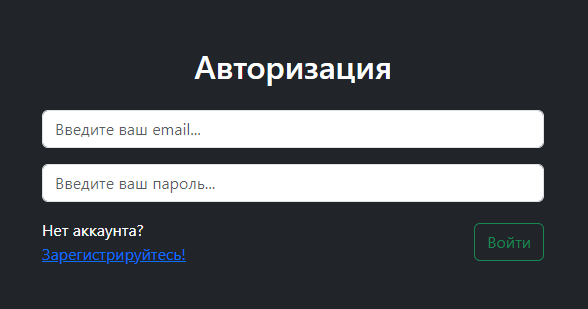
\includegraphics[width=0.7\linewidth]{images/log_web}
	\caption{Система в состоянии «Пользователь не аутентифицирован»}
	\label{fig:logweb}
\end{figure}

В случае наличия аутентификационных данных, пользователь сможет войти в систему. В случае отсутствия аутентификационных данных, пользователь может перейти к окну регистрации, нажав на соответствующую ссылку. Система в состоянии «Регистрация пользователя» представлена на рисунке \ref{fig:regweb}.

\begin{figure}[ht]
	\centering
	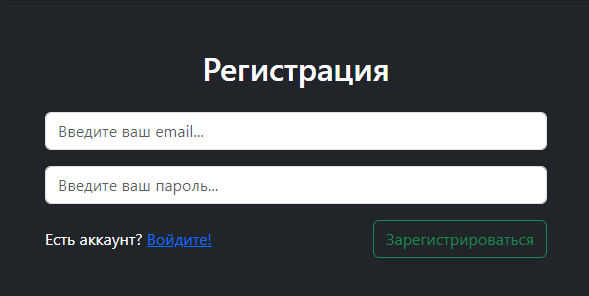
\includegraphics[width=0.7\linewidth]{images/reg_web}
	\caption{Система в состоянии «Регистрация пользователя»}
	\label{fig:regweb}
\end{figure}

После успешной регистрации пользователя переносит на главную страницу, где он может сам решить, что ему делать сначала. Данное состояние представлено на рисунке \ref{fig:mainweb}.

\begin{figure}[ht]
	\centering
	
\includegraphics[width=0.7\linewidth]{images/main_web}
	\caption{Система в состоянии «Главная страница»}
	\label{fig:mainweb}
\end{figure}

Арользователь решил посмотреть инфомрацию о себе и открыл профиль. Состояние «Профиль пользователя» представлен на рисунке \ref{fig:profileweb}.

\begin{figure}[ht]
	\centering
	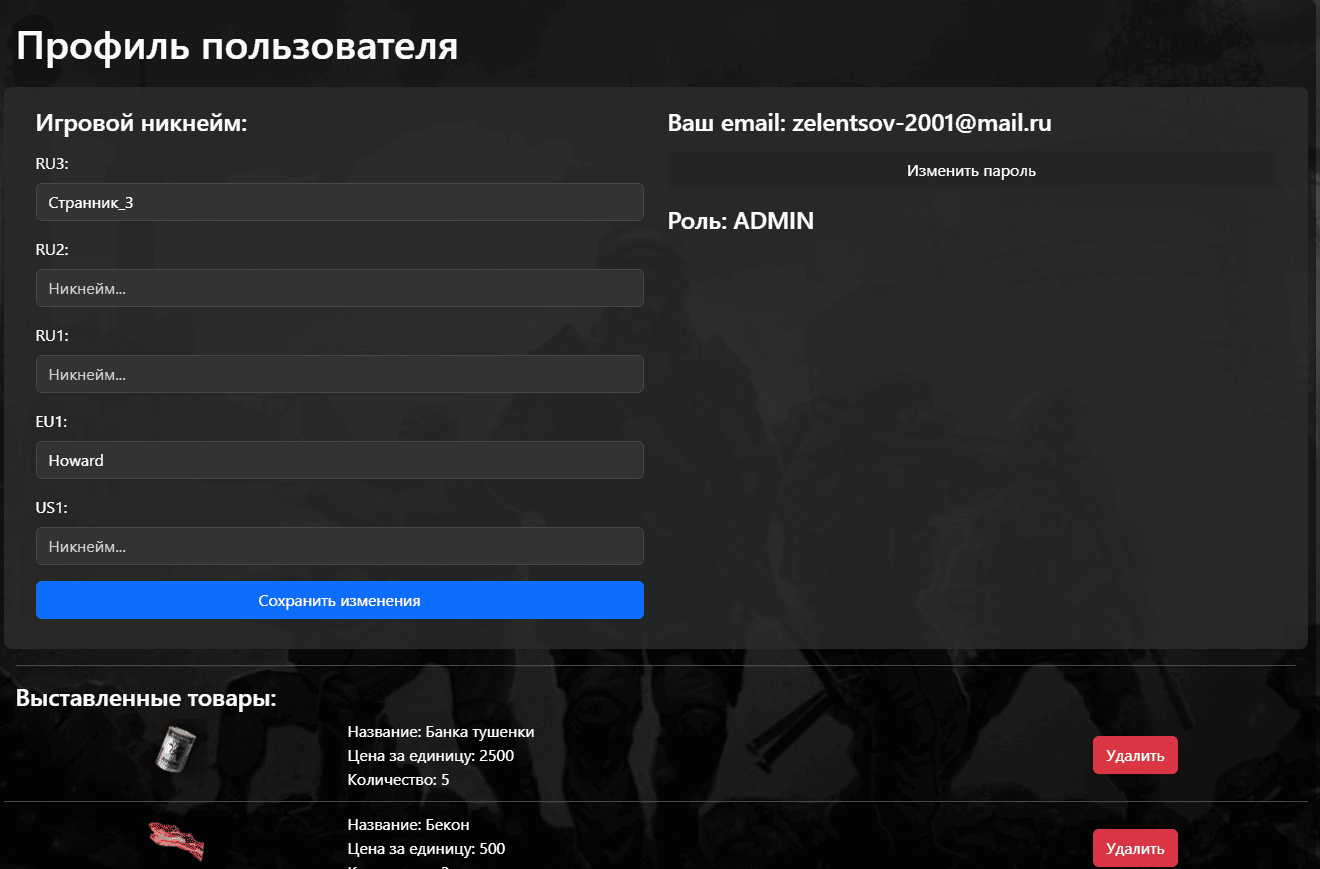
\includegraphics[width=0.7\linewidth]{images/profile_web}
	\caption{Система в состоянии «Профиль пользователя»}
	\label{fig:profileweb}
\end{figure}

После этого пользователь может поменять свой пароль на более надежный. Если введенный текущий пароль не правильный, то пользователь видит соответствующее сообщение. Если текущий пароль введен правильно, но новый пароль и повторный не совпадают, то пользователь видет соответствующее сообщение. Система в состоянии «Успешная смена пароля» представлена на рисунке \ref{fig:passwweb3}.

\begin{figure}[ht]
	\centering
	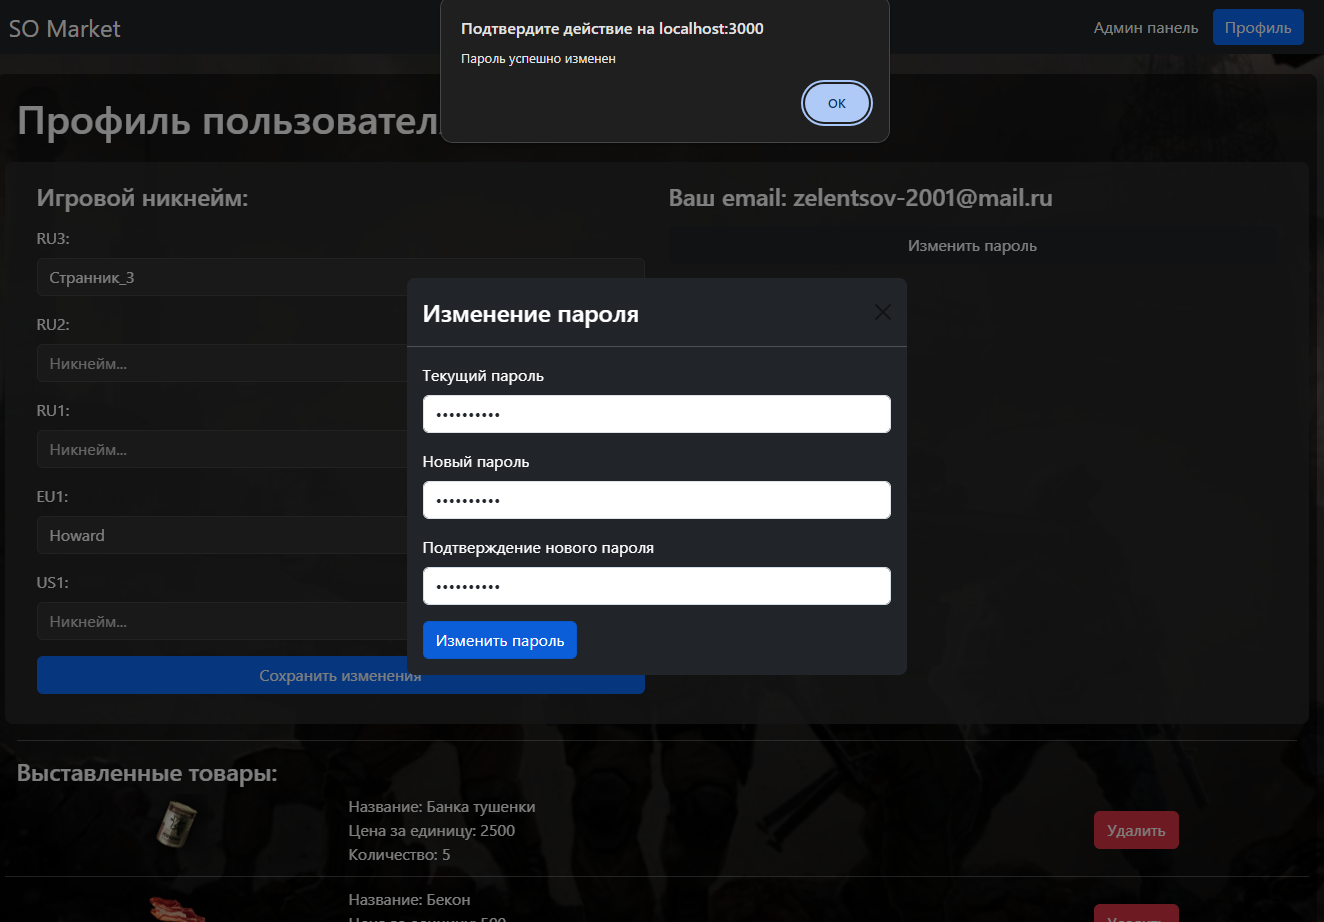
\includegraphics[width=0.7\linewidth]{images/passw_web3}
	\caption{Система в состоянии «Успешная смена пароля»}
	\label{fig:passwweb3}
\end{figure}

Система в состоянии «Неправильный текущий пароль» представлена на рисунке \ref{fig:passwweb1}.

\begin{figure}[ht]
	\centering
	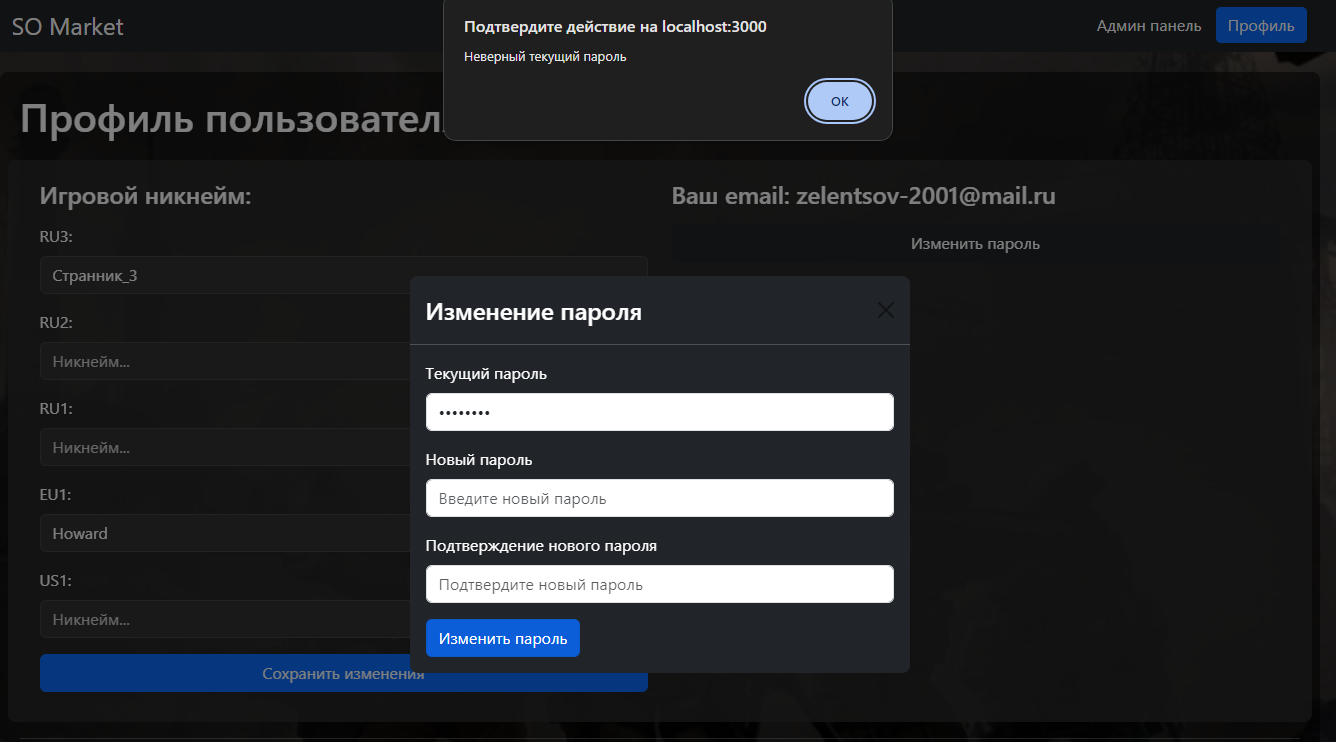
\includegraphics[width=0.7\linewidth]{images/passw_web1}
	\caption{Система в состоянии «Неправильный текущий пароль»}
	\label{fig:passwweb1}
\end{figure}

Система в состоянии «Новые пароли не совпадают» представлена на рисунке \ref{fig:passwweb2}.

\begin{figure}[ht]
	\centering
	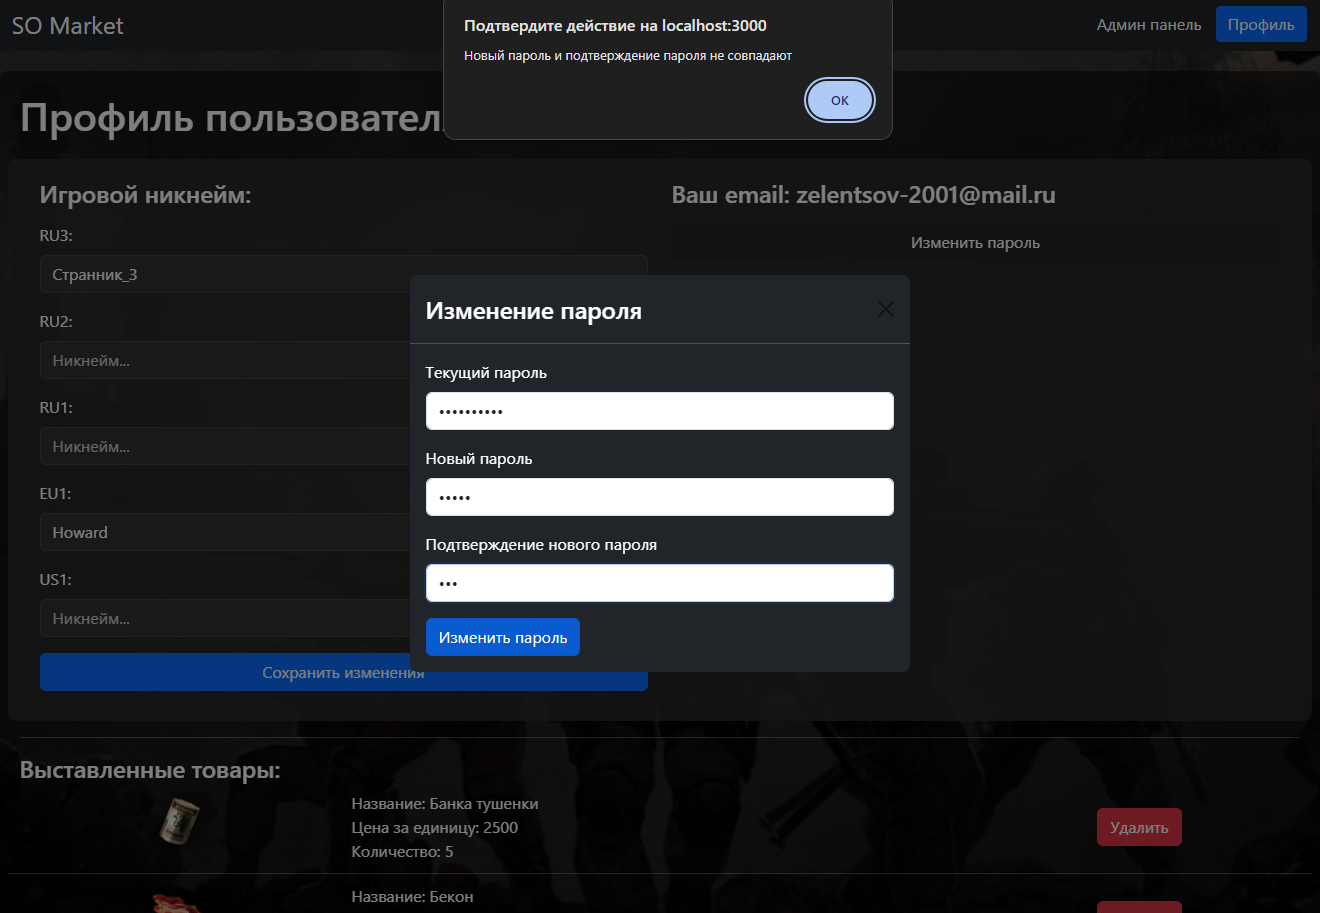
\includegraphics[width=0.7\linewidth]{images/passw_web2}
	\caption{Система в состоянии «Новые пароли не совпадают»}
	\label{fig:passwweb2}
\end{figure}

В профиле пользователь может установить свои игровые никнеймы. Система в этом состоянии представлена на рисунке \ref{fig:profilechangeweb}.

\begin{figure}[ht]
	\centering
	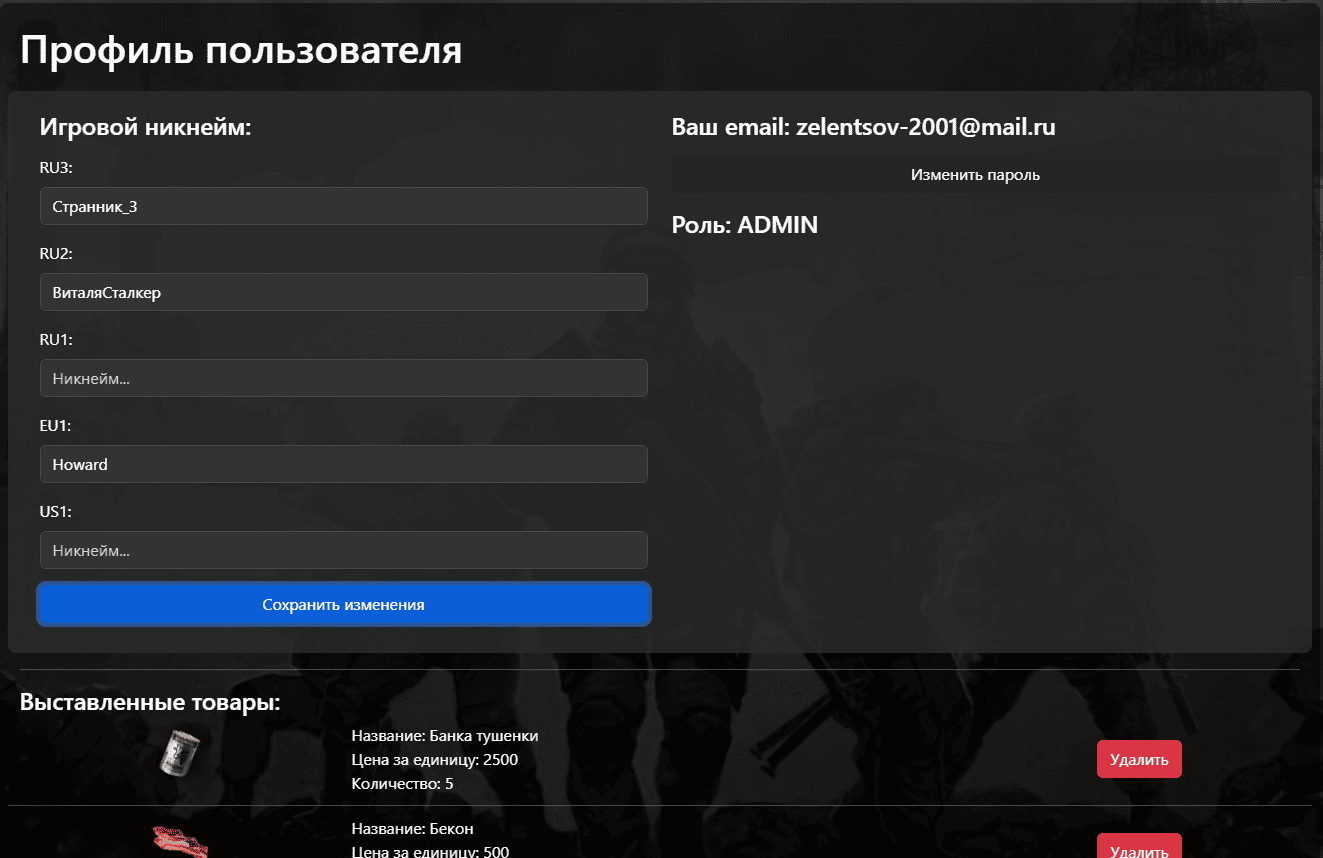
\includegraphics[width=0.7\linewidth]{images/profile_change_web}
	\caption{Система в состоянии «Сохранение никнейма»}
	\label{fig:profilechangeweb}
\end{figure}

Пользователь решил посмотреть, какие товары продают пользователи. Для этого ему необходимо выбрать интересующий его сервер. Система в этом состоянии представлена на рисунке \ref{fig:serverweb}.

\begin{figure}[ht]
	\centering
	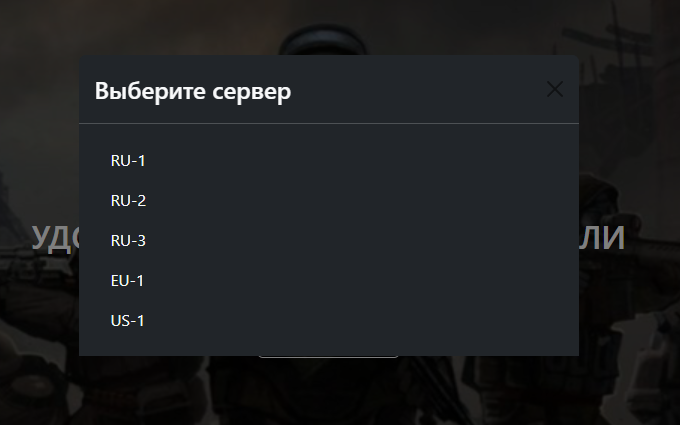
\includegraphics[width=0.7\linewidth]{images/server_web}
	\caption{Система в состоянии «Выбор сервера»}
	\label{fig:serverweb}
\end{figure}

После выбора сервера пользователь попадает на страницу с товарами. Система в этом состоянии представлена на рисунке \ref{fig:shopweb}.

\begin{figure}[ht]
	\centering
	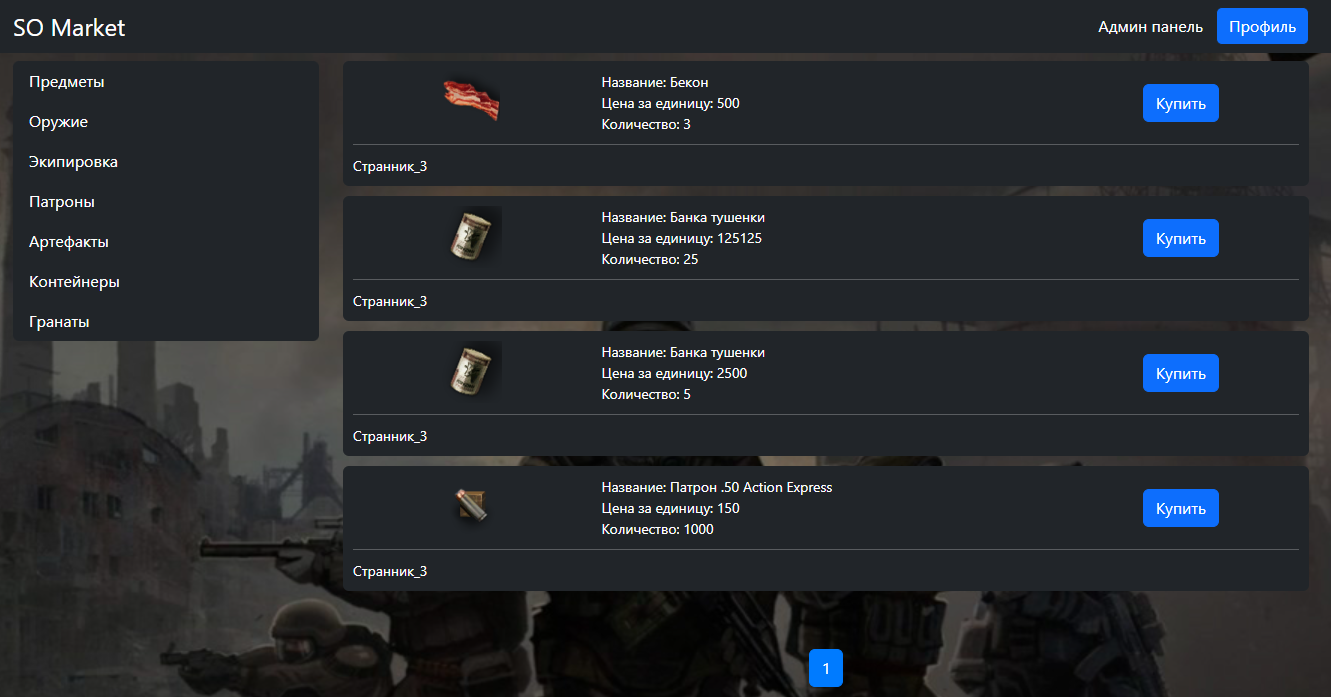
\includegraphics[width=0.7\linewidth]{images/shop_web}
	\caption{Система в состоянии «Отображение товаров»}
	\label{fig:shopweb}
\end{figure}

Пользователь может самостоятельно выбрать, какие товары отображать, установив параметры фильтрации. Система в этом состоянии представлена на рисунке \ref{fig:shopsortweb}.

\begin{figure}[ht]
	\centering
	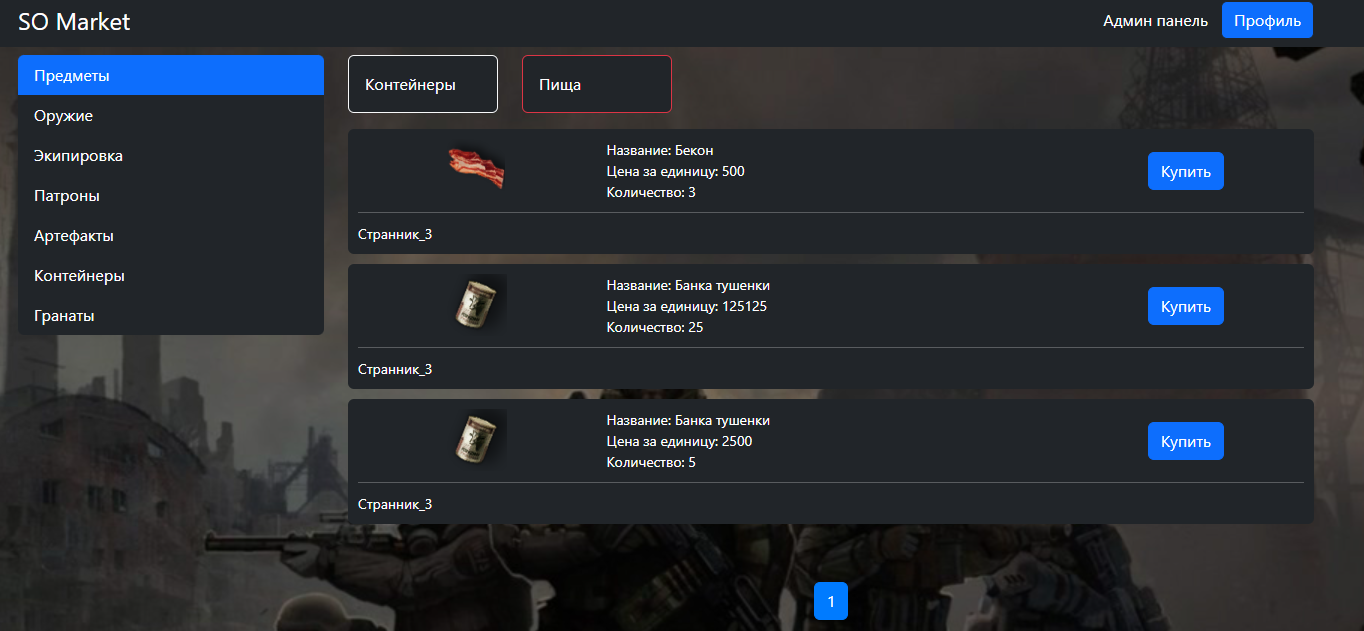
\includegraphics[width=0.7\linewidth]{images/shop_sort_web}
	\caption{Система в состоянии «Фильтрация товаров»}
	\label{fig:shopsortweb}
	
\end{figure}[ht]
Пользователь захотел сам выставить предмет на продажу. Для этого он нажимает на специальную кнопку и перед ним открывается форма. Система в состоянии «Выставить предмет на продажу» представлена на рисунке \ref{fig:sellweb}.

\begin{figure}[ht]
	\centering
	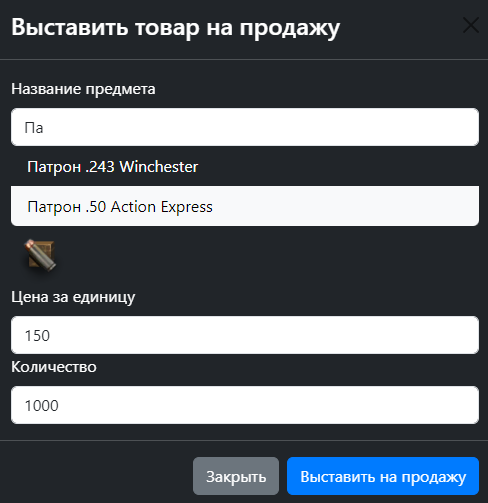
\includegraphics[width=0.6\linewidth]{images/sell_web}
	\caption{Система в состоянии «Выставить предмет на продажу»}
	\label{fig:sellweb}
	
\end{figure}[ht]
Пользователь с помощью поиска вводит название предмета, который он хочет продать и перед ним появляются все варианты, соответствующие введенным символам, вводит нужные количество предметов и их цену. Система в данном состоянии представлена на рисунке \ref{fig:sellonweb}.

\begin{figure}
	\centering
	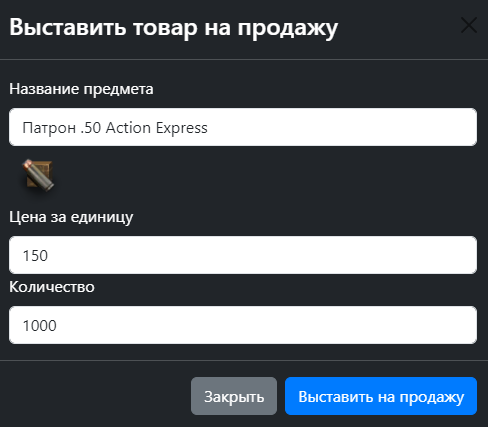
\includegraphics[width=0.7\linewidth]{images/sell_on_web}
	\caption{Система в состоянии «Продажа предмета»}
	\label{fig:sellonweb}
\end{figure}

Пользователь продал предмет или решил, что не хочет его продавать. Для этого он возвращается в профиль и нажимает на соответствующую кнопку в строке предмета. Система в этом состоянии представлена на рисунке \ref{fig:profileitemweb}.

\begin{figure}[ht]
	\centering
	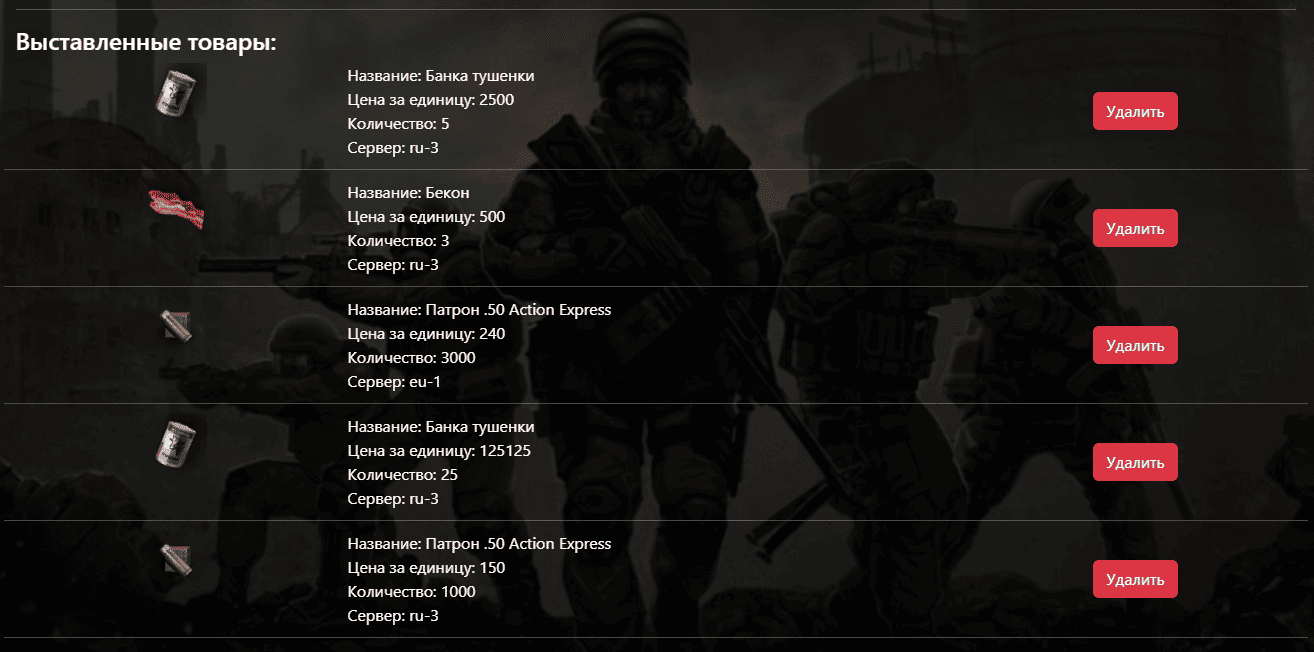
\includegraphics[width=0.7\linewidth]{images/profile_item_web}
	\caption{Система в состоянии «Отображение предметов пользователя»}
	\label{fig:profileitemweb}
\end{figure}

Пользователь решил посмотреть предметы на другом сервере. Для этого он переходит на главну юстраницу и выбирает другой сервер. Ему открывается ассортимент товаров с другого сервера. Система в данном состоянии представлена на рисунке \ref{fig:shopchangeweb}.

\begin{figure}[ht]
	\centering
	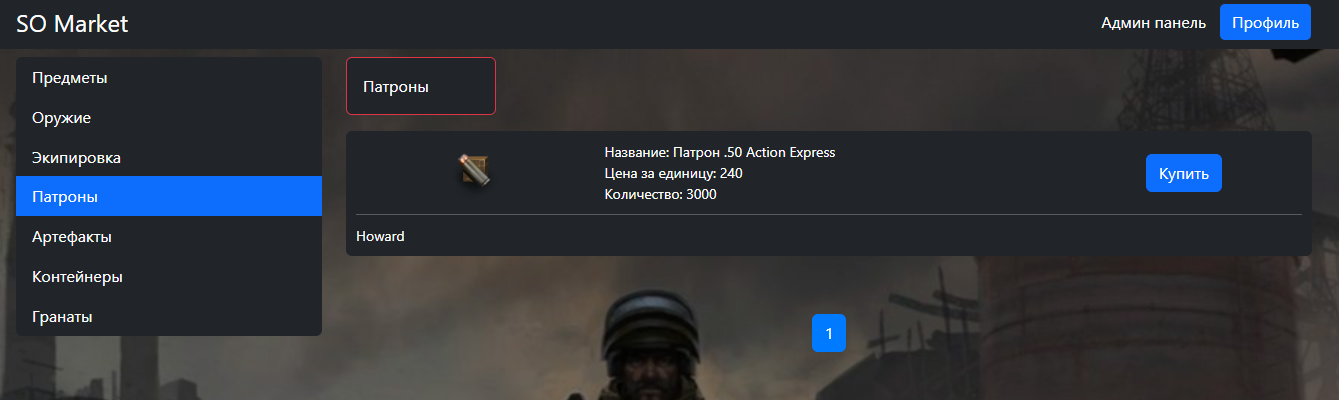
\includegraphics[width=0.7\linewidth]{images/shop_change_web}
	\caption{Система в состоянии «Отображение товаров другого сервера»}
	\label{fig:shopchangeweb}
\end{figure}

